\subsection{Insiemi}
\subsubsection{Cenni di teoria degli insiemi}
In generale supporremo validi gli assiomi su cui si fonda la teoria degli insiemi ZFC, ad eccezione dell'Assioma di Fondazione. Diamo innanzitutto una formulazione degli assiomi che interverranno nel seguito del lavoro:
\begin{axiom}[di estensionalità]
    Due insiemi sono uguali se e solo se contengono gli stessi elementi.
\end{axiom}

\begin{axiom}[di fondazione]
    Ogni insieme non vuoto contiene un elemento disgiunto dall'insieme stesso.
    \label{axi:foundation}
\end{axiom}
Del primo faremo un uso esplicito nel seguito. Il secondo, per motivi che saranno evidenti nella sezione seguente, risulta limitante nell'ambito che intendiamo trattare.

Vale la seguente definizione:
\begin{definition}
    Un insieme è \emph{ben-fondato} se non contiene se stesso. Altrimenti è \emph{non-ben-fondato}.
\end{definition}

\begin{example}
    L'insieme $\Omega = \{\Omega\}$ è non-ben-fondato. L'insieme $A = \{1,2,3\}$ è ben-fondato.
\end{example}

Riportiamo una formulazione equivalente dell'Assioma \ref{axi:foundation} \cite[Chapter III.4]{kunen}:
\begin{axiom*}[\ref{axi:foundation} bis]
    $\forall A$ la relazione ``$\in$'' è ben-fondata su $A$.
\end{axiom*}

Da questa formulazione risulta evidente l'impossibilità, nel sistema di assiomi ZFC, di costruire insiemi non-ben-fondati.

Rinunciando all'Assioma \ref{axi:foundation} si ottiene un sistema di assiomi che ammette l'esistenza di insiemi non-ben-fondati; tuttavia si può verificare che questo sistema non è più sufficiente a descrivere in modo esaustivo l'aritmetica per mezzo di operazioni su insiemi. Per ovviare a questa mancanza si introduce l'Assioma AFA, che verrà presentato e discusso nella sezione seguente.

% TODO: definisci insieme ereditariamente finito (si può costruire a partire dall'insieme vuoto utilizzando solamente il costruttore {} vedi ZFC) e insime non-ben-fondato prima di usare i grafi per rappresentare gli insiemi

\subsubsection{Rappresentazione di insiemi tramite grafi diretti}
\label{sec:graphs_sets}
In alcuni casi risulta conveniente fornire un'in\-ter\-pre\-ta\-zio\-ne insiemistica della nozione di grafo vista sopra. Introduciamo innanzitutto un concetto fondamentale per il seguito del lavoro:
\begin{definition}
    Sia $G = (V, E)$ un grafo diretto. Supponiamo che esista un $u \in V$ tale che ogni vertice del grafo è raggiungibile da $u$. Allora la coppia $(G, u)$ è un \emph{accessible pointed graph}, o \emph{APG}.
\end{definition}

Per rappresentare un insieme tramite un grafo diretto è necessario passare per un procedimento denominato \emph{decorazione}:
\begin{definition}
    La \emph{decorazione} di un APG è l'assegnazione di un insieme ad ogni suo nodo. In tal caso viene associata la relazione ``$\in$'' alla relazione $E$, ovvero $\langle a,b \rangle \iff b \in a$.
\end{definition}

Possiamo dare la seguente definizione:
\begin{definition}
    L'\emph{immagine} (o \emph{picture}) di un insieme $A$ è la coppia composta da un APG $(G,v)$ e da una sua decorazione in cui a $v$ è associato lo stesso $A$ \cite{aczel}.
\end{definition}

Vale la seguente proposizione \cite{aczel}:
\begin{proposition}
    Ad un APG aciclico è possibile associare un'unica decorazione.
\end{proposition}

Questo risultato non è stato dimostrato nel caso di un APG contenente almeno un ciclo. Per questo motivo viene introdotto il seguente assioma:
\begin{axiom}[AFA, Anti-Foundation-Axiom]
    Ogni APG possiede un'unica decorazione.
\end{axiom}

L'assioma AFA ha un'ovvia conseguenza:
\begin{corollary}
    Ogni APG è immagine di un unico insieme.
\end{corollary}

\begin{example}
    \begin{figure}[t]
        \centering
        \begin{subfigure}{.25\textwidth}
          \centering
          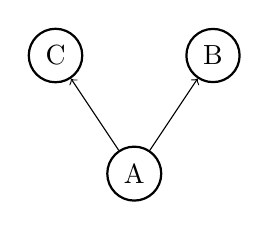
\begin{tikzpicture}[scale=0.5]
            \begin{scope}[every node/.style={circle,thick,draw}]
                \node (A) at (0,0) {A};
                \node (B) at (2,3) {B};
                \node (C) at (-2,3) {C};
            \end{scope}

            \begin{scope}
                \path [->] (A) edge node {} (B);
                \path [->] (A) edge node {} (C);
            \end{scope}
            \end{tikzpicture}
          \caption{$B = \{\emptyset\}$}
          \label{fig:sets_graphs_a}
        \end{subfigure}
        \begin{subfigure}{.15\textwidth}
            \centering
            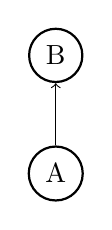
\begin{tikzpicture}[scale=0.5]
              \begin{scope}[every node/.style={circle,thick,draw}]
                  \node (A) at (0,0) {A};
                  \node (B) at (0,3) {B};
              \end{scope}

              \begin{scope}
                  \path [->] (A) edge node {} (B);
              \end{scope}
              \end{tikzpicture}
            \caption{$B = \{\emptyset\}$}
            \label{fig:sets_graphs_b}
          \end{subfigure}
        \begin{subfigure}{.15\textwidth}
          \centering
          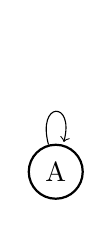
\begin{tikzpicture}[scale=0.5]
            \begin{scope}[every node/.style={circle,thick,draw}]
                \node (A) at (0,-0.3) {A};
                \node[draw=white] (B) at (0,3) {};
            \end{scope}

            \begin{scope}
                \path [->] (A) edge [loop above] node {} (A);
            \end{scope}
            \end{tikzpicture}
          \caption{$A = \{A\}$}
          \label{fig:sets_graphs_c}
        \end{subfigure}
        \begin{subfigure}{.25\textwidth}
            \centering
            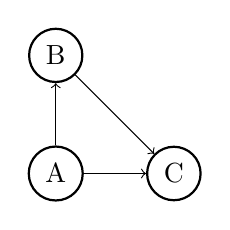
\begin{tikzpicture}[scale=0.5]
              \begin{scope}[every node/.style={circle,thick,draw}]
                  \node (A) at (0,0) {A};
                  \node (B) at (0,3) {B};
                  \node (C) at (3,0) {C};
              \end{scope}

              \begin{scope}
                  \path [->] (A) edge node {} (B);
                  \path [->] (B) edge node {} (C);
                  \path [->] (A) edge node {} (C);
              \end{scope}
              \end{tikzpicture}
            \caption{$A = \{\emptyset, \{\emptyset\}\}$}
            \label{fig:sets_graphs_d}
          \end{subfigure}

        \caption{Rappresentazione di insiemi tramite grafi.}
        \label{fig:graph_set}
    \end{figure}
    In Figura \ref{fig:graph_set} sono rappresentati alcuni insiemi sotto forma di APG. Nella Figura \ref{fig:sets_graphs_a} $B,C$ non hanno nodi figli, sicchè rappresentano l'insieme vuoto, e dunque $A$ è l'insieme che contiene solamente l'insieme vuoto; analogamente si interpreta la Figura \ref{fig:sets_graphs_b}; nella Figura \ref{fig:sets_graphs_c} abbiamo un nodo $A$ il cui unico figlio è lo stesso $A$, sicchè contiene solamente se stesso; infine nella Figura \ref{fig:sets_graphs_d} abbiamo un nodo $C$ che rappresenta l'insieme vuoto, un nodo $B$ che contiene solamente l'insieme vuoto, ed un nodo $A$ che contiene l'insieme vuoto è l'insieme rappresentato da $B$. Associazioni del tipo ``$B$ rappresenta l'insieme vuoto'' sono \emph{decorazioni}.
\end{example}
